
\documentclass[a4paper,12pt]{scrbook}
\usepackage{amsmath,amssymb,amsthm}
\usepackage{fancyvrb}
\usepackage{parskip}
\usepackage{lastpage}
\usepackage{verbatim,boxedminipage,enumitem}
\usepackage{ifthen}
\usepackage{color,graphicx}
\usepackage{pgf}
\usepackage{longtable}
\usepackage{upquote}
%\usepackage[all]{xy}
\usepackage{tobiShell}
\usepackage{tikz}
\usetikzlibrary{automata}
\usetikzlibrary{arrows}
\usepackage{pgf,pgfarrows,pgfnodes}
\usepackage{pgfplots}
\usepackage{circuitikz}
\usetikzlibrary{circuits}
\usetikzlibrary{circuits.logic.US}
\usepackage{mymath}
\usepackage{python}
%------------------------------------------------------------------
% Verbatim for console window - single line frame, no line numbers
%------------------------------------------------------------------
\DefineVerbatimEnvironment%
 {console}{Verbatim}
 {frame=single}

%--------------------------------------------------------
% Remove the vertical spacing before and after Verbatim.
%--------------------------------------------------------
\usepackage{atbeginend}
\BeforeBegin{console}{\mbox{}\\ \begin{minipage}{\textwidth}\vspace{3pt}}
\AfterEnd{console}{\vspace{4pt} \end{minipage} \\ }

\begin{document}
\thispagestyle{empty}

\begin{center}
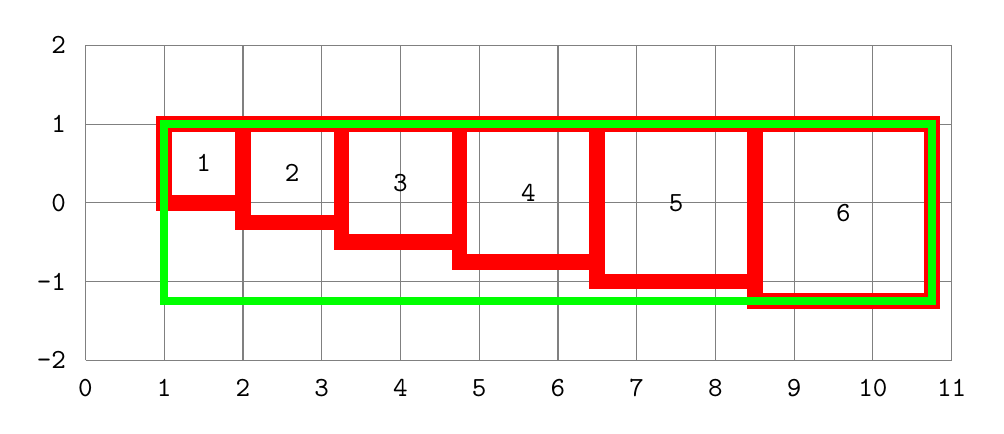
\begin{tikzpicture}
\draw[gray] (0.0,-2.0) to  (0.0,2.0);
\draw[gray] (1.0,-2.0) to  (1.0,2.0);
\draw[gray] (2.0,-2.0) to  (2.0,2.0);
\draw[gray] (3.0,-2.0) to  (3.0,2.0);
\draw[gray] (4.0,-2.0) to  (4.0,2.0);
\draw[gray] (5.0,-2.0) to  (5.0,2.0);
\draw[gray] (6.0,-2.0) to  (6.0,2.0);
\draw[gray] (7.0,-2.0) to  (7.0,2.0);
\draw[gray] (8.0,-2.0) to  (8.0,2.0);
\draw[gray] (9.0,-2.0) to  (9.0,2.0);
\draw[gray] (10.0,-2.0) to  (10.0,2.0);
\draw[gray] (11.0,-2.0) to  (11.0,2.0);
\draw[gray] (0.0,-2.0) to  (11.0,-2.0);
\draw[gray] (0.0,-1.0) to  (11.0,-1.0);
\draw[gray] (0.0,0.0) to  (11.0,0.0);
\draw[gray] (0.0,1.0) to  (11.0,1.0);
\draw[gray] (0.0,2.0) to  (11.0,2.0);
\draw(0, -2) node [font=\ttfamily, label=below:{\normalsize {\texttt{0}}}] {};
\draw(1, -2) node [font=\ttfamily, label=below:{\normalsize {\texttt{1}}}] {};
\draw(2, -2) node [font=\ttfamily, label=below:{\normalsize {\texttt{2}}}] {};
\draw(3, -2) node [font=\ttfamily, label=below:{\normalsize {\texttt{3}}}] {};
\draw(4, -2) node [font=\ttfamily, label=below:{\normalsize {\texttt{4}}}] {};
\draw(5, -2) node [font=\ttfamily, label=below:{\normalsize {\texttt{5}}}] {};
\draw(6, -2) node [font=\ttfamily, label=below:{\normalsize {\texttt{6}}}] {};
\draw(7, -2) node [font=\ttfamily, label=below:{\normalsize {\texttt{7}}}] {};
\draw(8, -2) node [font=\ttfamily, label=below:{\normalsize {\texttt{8}}}] {};
\draw(9, -2) node [font=\ttfamily, label=below:{\normalsize {\texttt{9}}}] {};
\draw(10, -2) node [font=\ttfamily, label=below:{\normalsize {\texttt{10}}}] {};
\draw(11, -2) node [font=\ttfamily, label=below:{\normalsize {\texttt{11}}}] {};
\draw(0, -2) node [font=\ttfamily, label=left:{\normalsize {\texttt{-2}}}] {};
\draw(0, -1) node [font=\ttfamily, label=left:{\normalsize {\texttt{-1}}}] {};
\draw(0, 0) node [font=\ttfamily, label=left:{\normalsize {\texttt{0}}}] {};
\draw(0, 1) node [font=\ttfamily, label=left:{\normalsize {\texttt{1}}}] {};
\draw(0, 2) node [font=\ttfamily, label=left:{\normalsize {\texttt{2}}}] {};

\draw (1.5, 0.5)
  node[draw, line width=0.2cm, , color=red,
       rounded corners=0cm, inner sep=0cm] {

\begin{minipage}[t][1.0cm]{1.0cm}
\mbox{}

\end{minipage}

};\draw (1.5, 0.5) node[color=black] {{\texttt{1}}};
\draw (2.625, 0.375)
  node[draw, line width=0.2cm, , color=red,
       rounded corners=0cm, inner sep=0cm] {

\begin{minipage}[t][1.25cm]{1.25cm}
\mbox{}

\end{minipage}

};\draw (2.625, 0.375) node[color=black] {{\texttt{2}}};
\draw (4.0, 0.25)
  node[draw, line width=0.2cm, , color=red,
       rounded corners=0cm, inner sep=0cm] {

\begin{minipage}[t][1.5cm]{1.5cm}
\mbox{}

\end{minipage}

};\draw (4.0, 0.25) node[color=black] {{\texttt{3}}};
\draw (5.625, 0.125)
  node[draw, line width=0.2cm, , color=red,
       rounded corners=0cm, inner sep=0cm] {

\begin{minipage}[t][1.75cm]{1.75cm}
\mbox{}

\end{minipage}

};\draw (5.625, 0.125) node[color=black] {{\texttt{4}}};
\draw (7.5, 0.0)
  node[draw, line width=0.2cm, , color=red,
       rounded corners=0cm, inner sep=0cm] {

\begin{minipage}[t][2.0cm]{2.0cm}
\mbox{}

\end{minipage}

};\draw (7.5, 0.0) node[color=black] {{\texttt{5}}};
\draw (9.625, -0.125)
  node[draw, line width=0.2cm, , color=red,
       rounded corners=0cm, inner sep=0cm] {

\begin{minipage}[t][2.25cm]{2.25cm}
\mbox{}

\end{minipage}

};\draw (9.625, -0.125) node[color=black] {{\texttt{6}}};
\draw (5.875, -0.125)
  node[draw, line width=0.1cm, , color=green,
       rounded corners=0cm, inner sep=0cm] {

\begin{minipage}[t][2.25cm]{9.75cm}
\mbox{}

\end{minipage}

};
\end{tikzpicture}

\end{center}

\end{document}
